\documentclass[]{article}
\usepackage{lmodern}
\usepackage{amssymb,amsmath}
\usepackage{ifxetex,ifluatex}
\usepackage{fixltx2e} % provides \textsubscript
\ifnum 0\ifxetex 1\fi\ifluatex 1\fi=0 % if pdftex
  \usepackage[T1]{fontenc}
  \usepackage[utf8]{inputenc}
\else % if luatex or xelatex
  \ifxetex
    \usepackage{mathspec}
  \else
    \usepackage{fontspec}
  \fi
  \defaultfontfeatures{Ligatures=TeX,Scale=MatchLowercase}
\fi
% use upquote if available, for straight quotes in verbatim environments
\IfFileExists{upquote.sty}{\usepackage{upquote}}{}
% use microtype if available
\IfFileExists{microtype.sty}{%
\usepackage{microtype}
\UseMicrotypeSet[protrusion]{basicmath} % disable protrusion for tt fonts
}{}
\usepackage[margin=1in]{geometry}
\usepackage{hyperref}
\hypersetup{unicode=true,
            pdftitle={Chapter 4: Numerical Integration Homework},
            pdfborder={0 0 0},
            breaklinks=true}
\urlstyle{same}  % don't use monospace font for urls
\usepackage{graphicx,grffile}
\makeatletter
\def\maxwidth{\ifdim\Gin@nat@width>\linewidth\linewidth\else\Gin@nat@width\fi}
\def\maxheight{\ifdim\Gin@nat@height>\textheight\textheight\else\Gin@nat@height\fi}
\makeatother
% Scale images if necessary, so that they will not overflow the page
% margins by default, and it is still possible to overwrite the defaults
% using explicit options in \includegraphics[width, height, ...]{}
\setkeys{Gin}{width=\maxwidth,height=\maxheight,keepaspectratio}
\IfFileExists{parskip.sty}{%
\usepackage{parskip}
}{% else
\setlength{\parindent}{0pt}
\setlength{\parskip}{6pt plus 2pt minus 1pt}
}
\setlength{\emergencystretch}{3em}  % prevent overfull lines
\providecommand{\tightlist}{%
  \setlength{\itemsep}{0pt}\setlength{\parskip}{0pt}}
\setcounter{secnumdepth}{5}
% Redefines (sub)paragraphs to behave more like sections
\ifx\paragraph\undefined\else
\let\oldparagraph\paragraph
\renewcommand{\paragraph}[1]{\oldparagraph{#1}\mbox{}}
\fi
\ifx\subparagraph\undefined\else
\let\oldsubparagraph\subparagraph
\renewcommand{\subparagraph}[1]{\oldsubparagraph{#1}\mbox{}}
\fi

%%% Use protect on footnotes to avoid problems with footnotes in titles
\let\rmarkdownfootnote\footnote%
\def\footnote{\protect\rmarkdownfootnote}

%%% Change title format to be more compact
\usepackage{titling}

% Create subtitle command for use in maketitle
\newcommand{\subtitle}[1]{
  \posttitle{
    \begin{center}\large#1\end{center}
    }
}

\setlength{\droptitle}{-2em}

  \title{Chapter 4: Numerical Integration Homework}
    \pretitle{\vspace{\droptitle}\centering\huge}
  \posttitle{\par}
  \subtitle{Joseph Sepich}
  \author{}
    \preauthor{}\postauthor{}
    \date{}
    \predate{}\postdate{}
  

\begin{document}
\maketitle

{
\setcounter{tocdepth}{2}
\tableofcontents
}
\section{Problem 1}\label{problem-1}

Data table for \(f(x) = e^{-x}, x \in [0,0.8]\)

\[
\begin{tabular}{c|c|c|c|c|c}
x & 0.0 & 0.2 & 0.4 & 0.6 & 0.8 \\
f(x) & 1 & 0.818731 & 0.670320 & 0.548812 & 0.449329
\end{tabular}
\]

\subsection{a. Write out the trapezoid rule and compute with 6
digits}\label{a.-write-out-the-trapezoid-rule-and-compute-with-6-digits}

Recall the trapezoid rule:

\[T(f;h) = h[\frac12f(x_0) + \Sigma f(x_i) + \frac12 f(x_n)]\]
\[T(e^{-x};0.2) = 0.2[\frac12(1)+\frac120.4493 + 0.8187 + 0.6703 + 0.5488]\]
\[T(e^{-x};0.2) = 0.552505\]

\subsection{b. Write out Simpson's rule and compute with 6
digits}\label{b.-write-out-simpsons-rule-and-compute-with-6-digits}

Recall Simpson's rule:

\[S(f;h) = \frac{h}3[f(x_0) + 4\Sigma f(x_{2i-1}) + 2\Sigma f(x_{2i}) + f(x_{2n})]\]
\[S(f;h) = 0.550676\]

\subsection{c. What is exact value of integral? What is each absolute
error? Which method is
better?}\label{c.-what-is-exact-value-of-integral-what-is-each-absolute-error-which-method-is-better}

Actual value is:

\[1-e^{-\frac45} = 0.550671\]

Abs error of Trapezoid is \(0.552505 - 0.550671 = 0.001834\), while
Simpson's rule had \(0.550676 - 0.550671 = 0.00005\). Simpson's method
clearly worked better in terms of error.

\subsection{\texorpdfstring{Given the error formula for each rule, how
many points would each method need for an error bound of
\(10^-4\)?}{Given the error formula for each rule, how many points would each method need for an error bound of 10\^{}-4?}}\label{given-the-error-formula-for-each-rule-how-many-points-would-each-method-need-for-an-error-bound-of-10-4}

Trapezoid Rule:

\[-\frac{0.8}{12}h^2e^{-0} \leq 10^{-4}\] \[h^2 \leq 15*10^{-4}\]
\[h \leq 0.038730\] \[n \geq 20.66 \]

This requires at least 22 points. Simpson's Rule:

\[-\frac{0.8}{180}h^4\leq 10^{-4}\] \[h^4 \leq 225 * 10^{-4}\]
\[h \leq 0.38730\] \[n \geq 1.033\]

This methods requires at least 5 points. Much less!

\section{Problem 2, Simpson's Rule}\label{problem-2-simpsons-rule}

\subsection{a. Calculate the given function on
{[}0,1{]}}\label{a.-calculate-the-given-function-on-01}

Recall the rule:

\[S(f;h) = \frac{h}3[f(x_0) + 4\Sigma f(x_{2i-1}) + 2\Sigma f(x_{2i}) + f(x_{2n})]\]
\[S(f;h) = 0.48\]

\subsection{\texorpdfstring{b. Tolerance is 10\textsuperscript{-6}. How
many points do you
need?}{b. Tolerance is 10-6. How many points do you need?}}\label{b.-tolerance-is-10-6.-how-many-points-do-you-need}

\[-\frac{1}{180}h^4(-1.25)\leq 10^{-6}\] \[h^4 \leq 144 * 10^{-6}\]
\[h \leq 0.1095445\] \[n \geq 9.129\]

For an error tolerance of 10\textsuperscript{-6}, Simpson's rule would
need at least 20 points.

\section{Problem 3, Trapezoid Rule and
Romberg}\label{problem-3-trapezoid-rule-and-romberg}

\subsection{a. Compute the trapezoid rule for the integral for n =
1,2}\label{a.-compute-the-trapezoid-rule-for-the-integral-for-n-12}

\[f(x) = 3x^2, [a,b] =[-1,1]\]

Recall the rule:

\[T(f;h) = h[\frac12f(x_0) + \Sigma f(x_i) + \frac12 f(x_n)]\]

n = 1 evaluates to 6

\[
\begin{tabular}{c|c|c}
x & -1 & 1 \\
f(x) & 3 & 3
\end{tabular}
\]

n = 2 evalutes to 3

\[
\begin{tabular}{c|c|c|c}
x & -1 & 0 & 1 \\
f(x) & 3 & 0 & 3
\end{tabular}
\]

\subsection{b. Evaluate with Romberg until you get the exact
value.}\label{b.-evaluate-with-romberg-until-you-get-the-exact-value.}

The exact value of x\textsuperscript{3} evaluated at {[}-1,1{]} is 2.

With n = 4 we now evalute to 2.25.

\[
\begin{tabular}{c|c|c|c|c|c}
x & -1 & -0.5 & 0 & 0.5 & 1 \\
f(x) & 3 & 0.75 & 0 & 0.75 & 3
\end{tabular}
\]

With n = 8 we then yield 2.0625. With n = 16 we then yield 2.015625.
With n = 32 we then yield 2.003906, so we are getting closer, but we are
not getting the exact value.

\subsection{c.}\label{c.}

w = 1 and a = 0.577350 (or 1/\(\sqrt3\)) works for any polynomial of
degree 3 or less. We derived this in lecture.

\section{Problem 4}\label{problem-4}

Trapezoid Function:

\begin{verbatim}
function v=trapezoid(fun,a,b,n)
%TRAPEZOID numerical integration by trapezoid rule
h=(b-a)/n;
xi=a:h:b;
v = h*(0.5*feval(fun,xi(1))+sum(feval(fun,xi(2:1:end-1)))+0.5*feval(fun,(xi(end))));
end
\end{verbatim}

Script:

\begin{verbatim}
n = [4 8 16 32 64 128];
actual = 0.550676;
absErr = zeros(1,length(n));

for i = 1:length(n)
    % func is e^-x
   val = trapezoid('func',0,0.8,n(i));
   absErr(i) = val - actual;
   disp(val)
end

figure
loglog(n, absErr)
title('Absolute Error in trapezoid rule')
xlabel('Number of segments')
ylabel('Absolute Error')
\end{verbatim}

And figure 1 is the plot of the error:

\begin{figure}
\centering
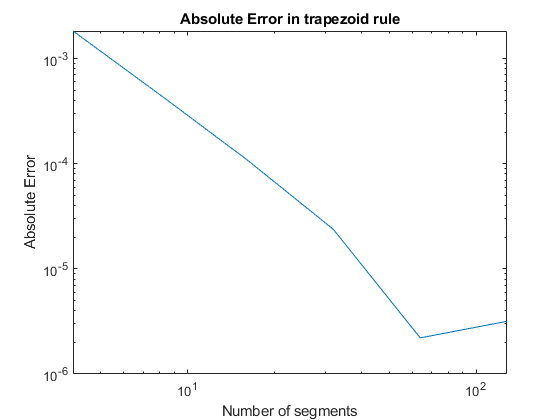
\includegraphics{./ch4prob4.png}
\caption{}
\end{figure}

When n is doubled the error value appears to cut by a factor of 4 times.

\section{Problem 5}\label{problem-5}

Simpson Function:

\begin{verbatim}
function v=Simpson(fun,a,b,n)
%SIMPSON numerical integration using simpson's rule
    h=(b-a)/n; xi=a:h:b;
    v= h/3*(feval(fun,xi(1))+2*sum(feval(fun,xi(3:2:end-2)))+4*sum(feval(fun,xi(2:2:end)))+feval(fun,xi(end)));
end
\end{verbatim}

Script:

\begin{verbatim}
n = [2 4 8 16 32 128];
actual = 0.550676;
absErr = zeros(1,length(n));

for i = 1:length(n)
    % func is e^-x
   val = Simpson('func',0,0.8,n(i));
   absErr(i) = abs(val - actual);
   disp(val)
end

figure
loglog(n, absErr)
title('Absolute Error in trapezoid rule')
xlabel('Number of segments')
ylabel('Absolute Error')
\end{verbatim}

When n is doubled here, at least from n = 2 to n = 4, the error is
decreased about 70 times.

Figure 2 is the plot:

\begin{figure}
\centering
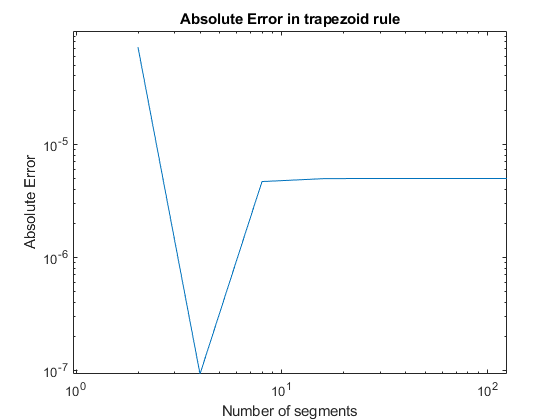
\includegraphics{./ch4prob5.png}
\caption{}
\end{figure}

\section{Problem 6}\label{problem-6}

Romberg script:

\begin{verbatim}
function r = romberg(fun,a,b,n)
h = (b - a) ./ (2.^(0:n-1));
r(1,1) = (b - a) * (feval(fun,a) + feval(fun,b)) / 2;
for j = 2:n
    subtotal = 0;
    for i = 1:2^(j-2)
        subtotal = subtotal + feval(fun,a + (2 * i - 1) * h(j));
    end
    r(j,1) = r(j-1,1) / 2 + h(j) * subtotal;
    for k = 2:j
        r(j,k) = (4^(k-1) * r(j,k-1) - r(j-1,k-1)) / (4^(k-1) - 1);
    end
end
\end{verbatim}

Function files:

\begin{verbatim}
function v=func(x)
    %v = exp(-1.*x);
    %v = cos(2.*x).*exp(-1.*x);
    v = sin(x);
    %v = x.^0.5;
end

function v=f(x)
    %v = exp(-1.*x);
    %v = cos(2.*x).*exp(-1.*x);
    %v = sin(x);
    v = x.^0.5;
end
\end{verbatim}

Script file

\begin{verbatim}
rows = 5;
vals = romberg('func',0,pi,rows);
act = 2;

format short e;
disp(vals)
for i = 1:rows
    for j = 1:rows
        if vals(i,j) == 0
            continue
        else
            vals(i,j) = vals(i,j) - act;
        end
    end
end

disp('First Function Error')
disp(vals)

rows = 5;
vals = romberg('f',0,1,rows);
act = 2/3;
disp(vals)
for i = 1:rows
    for j = 1:rows
        if vals(i,j) == 0
            continue
        else
            vals(i,j) = vals(i,j) - act;
        end
    end
end

disp('Second Function Error')
disp(vals)
\end{verbatim}

Tables in figure 3:

\begin{figure}
\centering
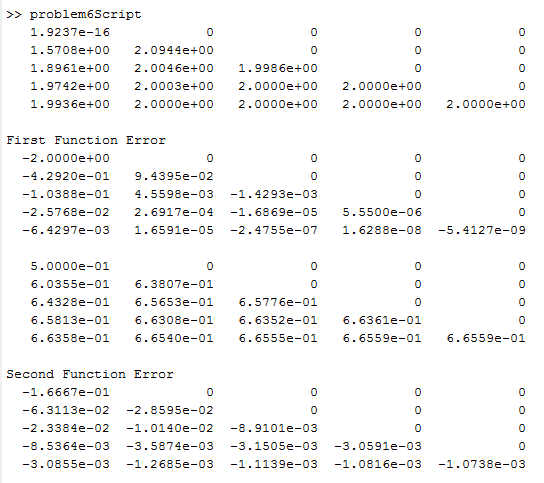
\includegraphics{./ch4prob6.png}
\caption{}
\end{figure}

q = quad(`f',0,1,1e-9)

q =

\begin{quote}
\begin{quote}
6.6667e-01
\end{quote}
\end{quote}

w = quad(`func',0,pi,1e-9)

w =

\begin{quote}
\begin{quote}
2.0000e+00
\end{quote}
\end{quote}

q = quadl(`f',0,1,1e-9)

q =

\begin{quote}
\begin{quote}
6.6667e-01
\end{quote}
\end{quote}

w = quadl(`func',0,pi,1e-9)

w =

\begin{quote}
\begin{quote}
2.0000e+00
\end{quote}
\end{quote}

These quadrature approaches are spot on.

\section{Problem 7}\label{problem-7}

\subsection{a. Calculate J at n = 1,3,9}\label{a.-calculate-j-at-n-139}

I use the trapezoid formula:

\[T(f;h) = h[\frac12f(x_0) + \Sigma f(x_i) + \frac12 f(x_n)]\]

\begin{verbatim}
n = [1 3 9];

for i = 1:length(n)
    space = 1 / n(i);
    x = 0:space:1;
    y = zeros(1,length(x));
    y(1) = 1;
    y(2:end) = func(x(2:end));
    val = trapz(space,y);
    disp(val)
end
\end{verbatim}

Gives us:

\[
\begin{tabular}{c|c|c|c}
n & 1 & 3 & 9 \\
J & 0.9207355 & 0.9432914 & 0.9457732
\end{tabular}
\]

I use my romberg fomula:

\begin{verbatim}
function r = romberg(fun,a,b,n)
h = (b - a) ./ (2.^(0:n-1));
r(1,1) = (b - a) * (feval(fun,a) + feval(fun,b)) / 2;
for j = 2:n
    subtotal = 0;
    for i = 1:2^(j-2)
        subtotal = subtotal + feval(fun,a + (2 * i - 1) * h(j));
    end
    r(j,1) = r(j-1,1) / 2 + h(j) * subtotal;
    for k = 2:j
        r(j,k) = (4^(k-1) * r(j,k-1) - r(j-1,k-1)) / (4^(k-1) - 1);
    end
end
\end{verbatim}

Gives us figure 4:

\begin{figure}
\centering
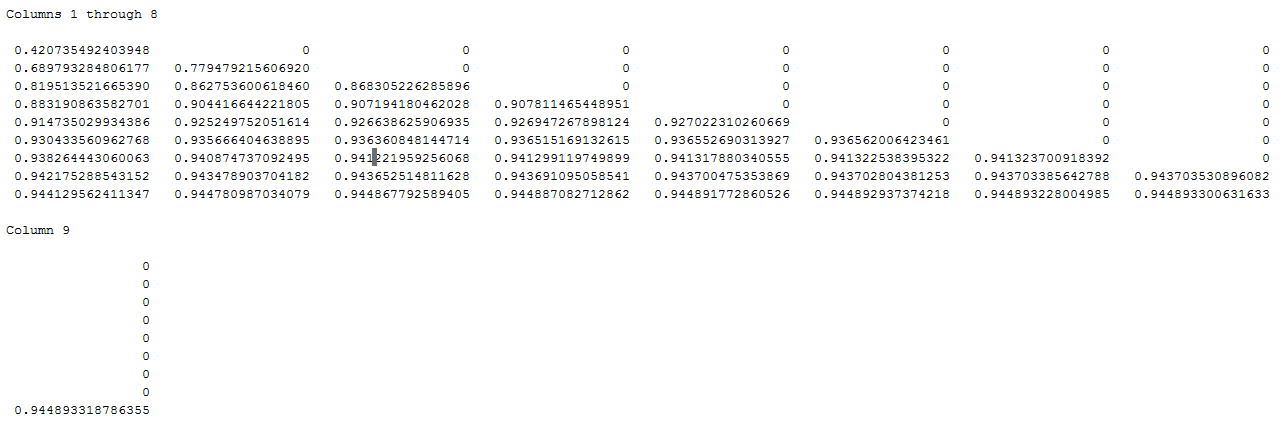
\includegraphics{./ch4prob7.png}
\caption{}
\end{figure}

\section{Problem 8}\label{problem-8}

\subsection{a.}\label{a.}

We want to assure that this quadrature gives us the exact value for any
polynomial of degree 7 or less.

Let's check:

f(x) = 1, The actual value from {[}-1,1{]} is 2, x is 0,
x\textsuperscript{2} is 2/3, x\textsuperscript{3} is 0,
x\textsuperscript{4} is 2/5, x\textsuperscript{5} is 0,
x\textsuperscript{6} is 2/7, and x\textsuperscript{7} is 0.

Using the values in matlab we get the following printout:

\begin{verbatim}
x = [-((3 - 4 * 0.3 ^ 5) / 7)^0.5 -((3 + 4 * 0.3 ^ 5) / 7)^0.5 ((3 - 4 * 0.3 ^ 5) / 7)^0.5 ((3 + 4 * 0.3 ^ 5) / 7)^0.5]
\end{verbatim}

\begin{quote}
\begin{quote}
-0.653592271330420 -0.655713352006805 0.653592271330420
0.655713352006805
\end{quote}
\end{quote}

\begin{verbatim}
a = [0.5 + (10/3)^0.5 / 12 0.5 - (10/3)^0.5 / 12 0.5 + (10/3)^0.5 / 12 0.5 - (10/3)^0.5 / 12]
\end{verbatim}

\begin{quote}
\begin{quote}
0.652145154862546 0.347854845137454 0.652145154862546 0.347854845137454
\end{quote}
\end{quote}

a(1)+a(2)+a(3)+a(4)

ans =

\begin{quote}
\begin{quote}
\begin{verbatim}
2
\end{verbatim}
\end{quote}
\end{quote}

a(1)\emph{x(1) + a(2)}x(2) + a(3)\emph{x(3) + a(4)}x(4)

ans =

\begin{quote}
\begin{quote}
-5.551115123125783e-17
\end{quote}
\end{quote}

a(1)\emph{x(1)\^{}2 + a(2)}x(2)\^{}2 + a(3)\emph{x(3)\^{}2 +
a(4)}x(4)\^{}2

ans =

\begin{quote}
\begin{quote}
0.856297799482706
\end{quote}
\end{quote}

a(1)\emph{x(1)\^{}3 + a(2)}x(2)\^{}3 + a(3)\emph{x(3)\^{}3 +
a(4)}x(4)\^{}3

ans =

\begin{quote}
\begin{quote}
-1.387778780781446e-17
\end{quote}
\end{quote}

a(1)\emph{x(1)\^{}4 + a(2)}x(2)\^{}4 + a(3)\emph{x(3)\^{}4 +
a(4)}x(4)\^{}4

ans =

\begin{quote}
\begin{quote}
0.366626459899463
\end{quote}
\end{quote}

a(1)\emph{x(1)\^{}5 + a(2)}x(2)\^{}5 + a(3)\emph{x(3)\^{}5 +
a(4)}x(4)\^{}5

ans =

\begin{quote}
\begin{quote}
\begin{verbatim}
0
\end{verbatim}
\end{quote}
\end{quote}

a(1)\emph{x(1)\^{}6 + a(2)}x(2)\^{}6 + a(3)\emph{x(3)\^{}6 +
a(4)}x(4)\^{}6

ans =

\begin{quote}
\begin{quote}
0.156973714736308
\end{quote}
\end{quote}

a(1)\emph{x(1)\^{}7 + a(2)}x(2)\^{}7 + a(3)\emph{x(3)\^{}7 +
a(4)}x(4)\^{}7

ans =

\begin{quote}
\begin{quote}
\begin{verbatim}
0
\end{verbatim}
\end{quote}
\end{quote}

\subsection{b.}\label{b.}

If we want our polynomial to be correct for all polynomials for degree
less than or equal to two we can set up a system of equations to find
our uknowns:

\[f(x) = 1 : a_1 + a_2 + a_3 = 2\]
\[f(x) = x: -0.5*a_1 + 0*a_2 + 0.5*a_3 = 0\]
\[f(x) = x^2: -0.5*a_1 + 0*a_2 + 0.5*a_3 = \frac23\]

Now solve!

\[a_1 + a_2 + a_3= 2\] \[-0.5a_1 + 0.5a_3 = 0\]
\[-0.5a_1+0.5a_3 = \frac23\]

We can add the second and third:

\[a_3 = \frac23\]

Plug back into number 2:

\[-\frac12a_1 = -\frac12\frac23\] \[a_1 = \frac23\]

Plugging into the first equation we have:

\[\frac23 + a_2 + \frac23 = 2\] \[a_2 + \frac43 = 2\]
\[a_2 = \frac63 - \frac43\] \[a-2 = \frac23\]

So all three values \(a_1, a_2, a_3 = \frac23\).


\end{document}
